% Templates
\begin{comment}

\begin{figure}[H]
	\centering
	\includegraphics[width=0.7\textwidth]{tyristor/}
	\caption{}
	\label{fig:}
\end{figure}

\vspace{0.5cm} % Add space after the solution

\begin{enumerate}[label=\roman*)]
	\item
	\item
\end{enumerate}

\end{comment}

\begin{question}[name=Spørsmål, topic=tyristor]
	En tyristor kan brukes som bryter. Styrestrømmen til tyristoren kan komme fra en impulsbryter. Hvordan skal strømmen gjennom tyristoren slåes av?
\end{question}

\vspace{0.5cm} % Add space after the solution

\begin{solution}[name=Løsningsforslag]
	Ved å bryte hovedstrømmen
\end{solution}

\vspace{0.5cm} % Add space after the solution

\begin{question}[name=Spørsmål, topic=tyristor]
Beskriv hva hovedforskjellen i virkemåten er mellom en tyristor og transistor
\end{question}

\vspace{0.5cm} % Add space after the solution

\begin{solution}[name=Løsningsforslag]
En tyristor kan kun ha diskrete tilstander, det vil si enten på eller av, mens en transistor kan operere kontinuerlig i mellomliggende tilstander og brukes til å regulere forsterkningen.
\end{solution}


\begin{question}[name=Spørsmål, topic=tyristor]
Kretsen som vist i Figur \ref{fig:tyrTriggplot} viser en spenningskilde koblet til en tyristor, som igjen er koblet til en last angitt som $R$. Tyristorens gate blir trigget av en puls som vist i \ref{fig:tyrForTriggplot}. Tegn hvordan spenningen over lasten $R$ vil endre seg som et produkt av tiden.
\begin{figure}[H]
	\centering
	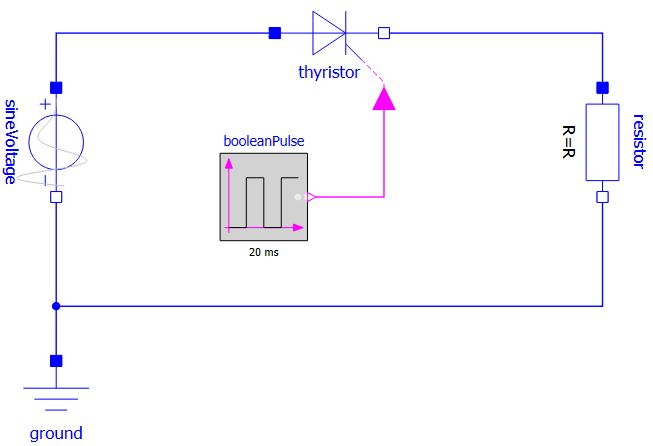
\includegraphics[width=0.7\textwidth]{tyristor/figurer/tyristor.png}
	\caption{Tyristor med trigger-signal}
	\label{fig:tyrTriggplot}
\end{figure}

\begin{figure}[H]
	\centering
	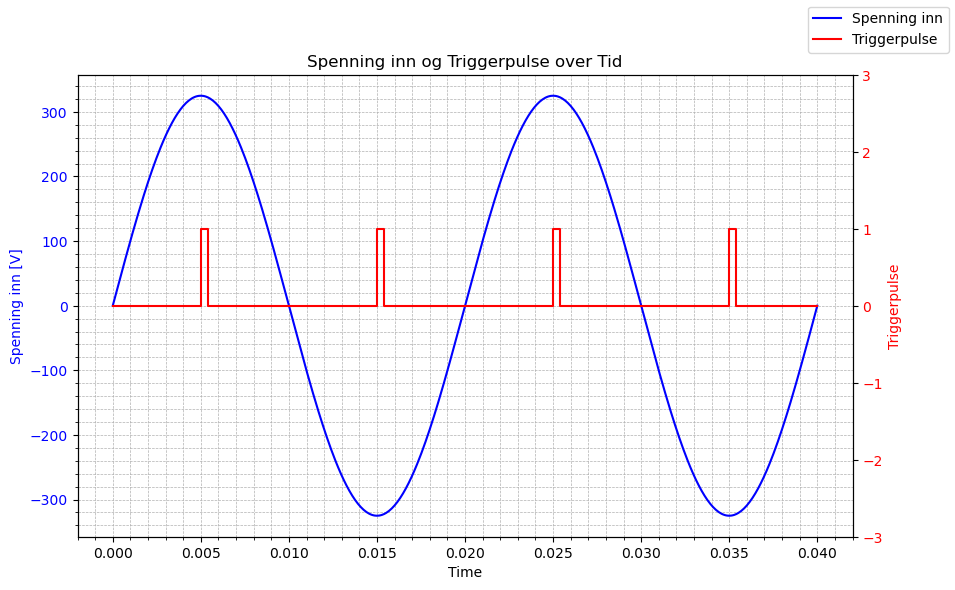
\includegraphics[width=0.7\textwidth]{tyristor/plot/tyristor3.png}
	\caption{Forløp for spenningskilde og trigger-signal}
	\label{fig:tyrForTriggplot}
\end{figure}


\end{question}

\vspace{0.5cm} % Add space after the solution

\begin{solution}[name=Løsningsforslag]
I Figur \ref{fig:tyrTriggplotSOL} kan man se hvordan tyristoren starter å lede kun når den blir trigget i positiv halvperiode. Detter er vist med det lilla arealet. Tyristoren slutter å lede ved nullgjennomgangen og starter ikke å lede før den blir trigget på nytt.

\begin{figure}[H]
	\centering
	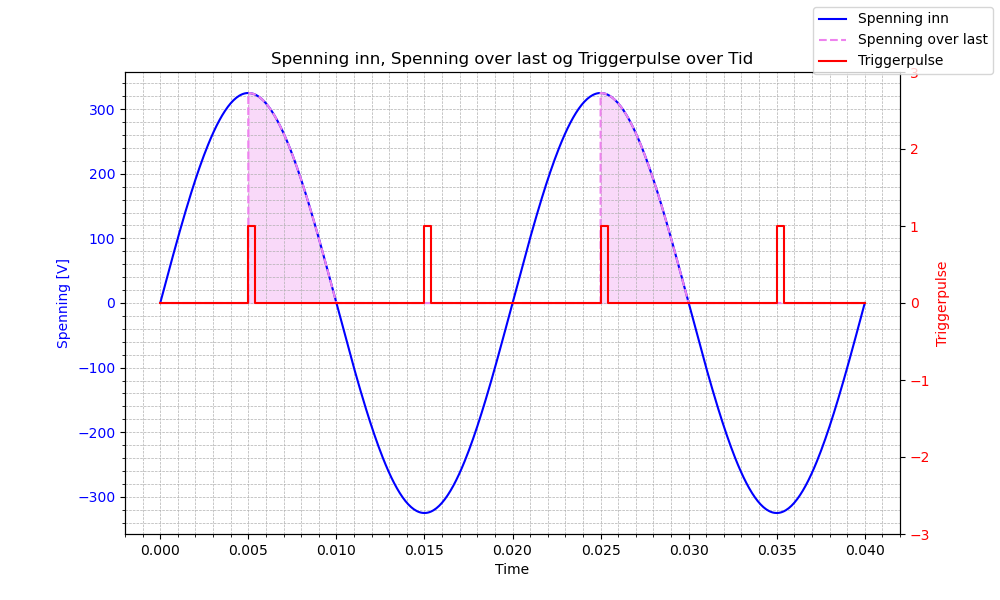
\includegraphics[width=0.9\textwidth]{tyristor/plot/tyristor3SOL.png}
	\caption{Tyristor med trigger-signal og spenning over last}
	\label{fig:tyrTriggplotSOL}
\end{figure}

\end{solution}



% ------------------- TRIAC -------------------


\begin{question}[name=Spørsmål, topic=tyristor]


	\begin{enumerate}[label=\roman*)]
		\item Hva står TRIAC for?
		\item Beskriv hva en TRIAC er
		\item Hva er det viktigste bruksområdene for TRIAC?

	\end{enumerate}
\end{question}



\vspace{0.5cm} % Add space after the solution

\begin{solution}[name=Løsningsforslag]


	\begin{enumerate}[label=\roman*)]
	\item Triode for Alternating Current
	\item En TRIAC er en halvlederkomponent som kan lede strøm i begge retninger. Den består av to tyristorer koblet i parallell, men i motsatt retning også kalt antiparallell
	\item TRIAC-er brukes ofte i vekselstrømskretser for å kontrollere strømmen til laster som motorer, lysdimmere og varmeelementer

\end{enumerate}




\end{solution}




\begin{question}[name=Spørsmål, topic=tyristor]
Beskriv funksjon til TRIAC koblingen i kretsen som vist i Figur \ref{fig:triPush}.
\begin{figure}[H]
	\centering
	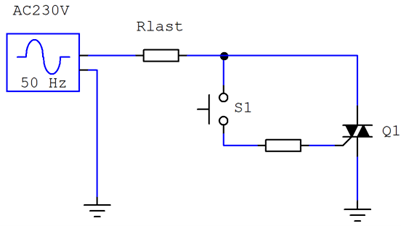
\includegraphics[width=0.6\textwidth]{tyristor/figurer/tricBasic.png}
	\caption{TRIAC krets med impulsbryter}
	\label{fig:triPush}
\end{figure}
\end{question}

\vspace{0.5cm} % Add space after the solution

\begin{solution}[name=Løsningsforslag]
TRIAC koblingen sørger for at man kan styre en større strøm ved hjelp av signal som trekker en mindre strøm.

TRIAC koblingen sørger for at kretsen blir brutt ved nullgjennomgangen som er spesielt fordelaktig når man bryter induktive kretser som potensielt vil kunne generere høy spenning og skade utstyret. Dette oppstår siden spenningen over en induktans er proporsjonal til endringsraten av strømmen gjennom induktansen, som vist i Formel \ref{eq:strømInd}.

\begin{equation}
	\label{eq:strømInd}
	U_{ind}=L \cdot \frac{dI_{ind}}{dt}
\end{equation}

\end{solution}


\begin{question}[name=Spørsmål, topic=tyristor]
	Kretsen som vist i Figur \ref{fig:triacTriggplot} viser en spenningskilde koblet til en TRIAC, som igjen er koblet til en last angitt som $R$. TRIAC-ens gate blir trigget av en puls som vist i \ref{fig:triacForTriggplot}. Tegn hvordan spenningen over lasten $R$ vil endre seg som et produkt av tiden.
	\begin{figure}[H]
		\centering
		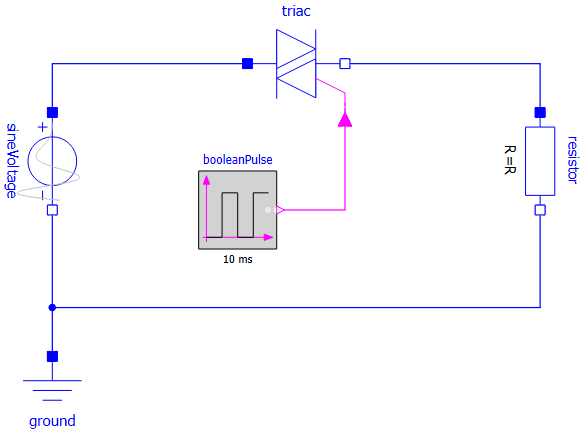
\includegraphics[width=0.5\textwidth]{tyristor/figurer/triac.png}
		\caption{TRIAC med trigger-signal}
		\label{fig:triacTriggplot}
	\end{figure}

	\begin{figure}[H]
		\centering
		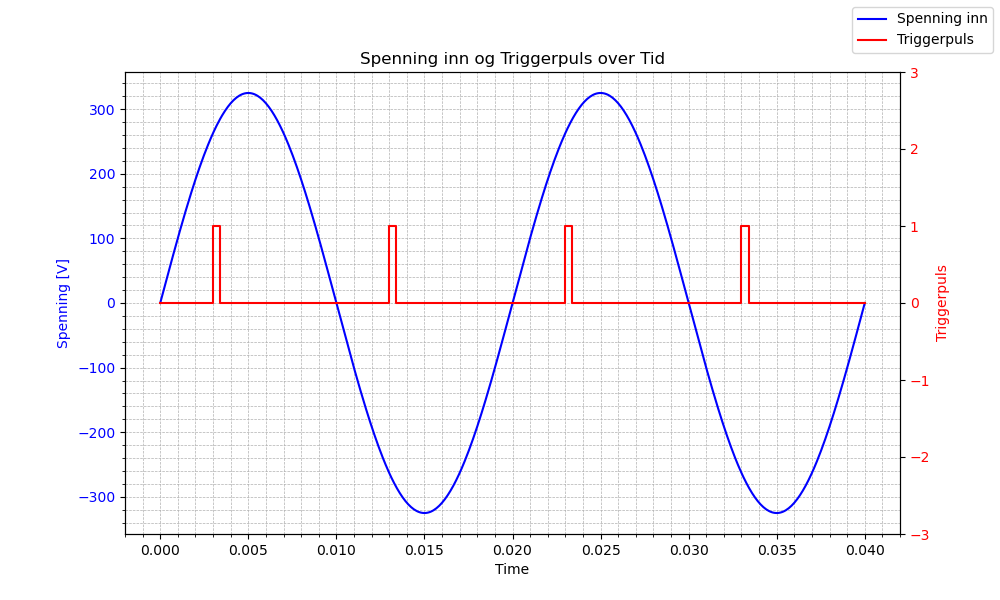
\includegraphics[width=0.7\textwidth]{tyristor/plot/triac.png}
		\caption{Forløp for spenningskilde og trigger-signal}
		\label{fig:triacForTriggplot}
	\end{figure}


\end{question}

\vspace{0.5cm} % Add space after the solution

\begin{solution}[name=Løsningsforslag]
	I Figur \ref{fig:triacTriggplotSOL} kan man se hvordan TRIAC-en starter å lede kun når den blir trigget. Siden en TRIAC er to tyristorer i anti-parallell vil TRIAC-en kunne lede for både positive og negative halvperioder. Detter er vist med det lilla arealet. TRIAC-en slutter å lede ved nullgjennomgangen og starter ikke å lede før den blir trigget på nytt.

	\begin{figure}[H]
		\centering
		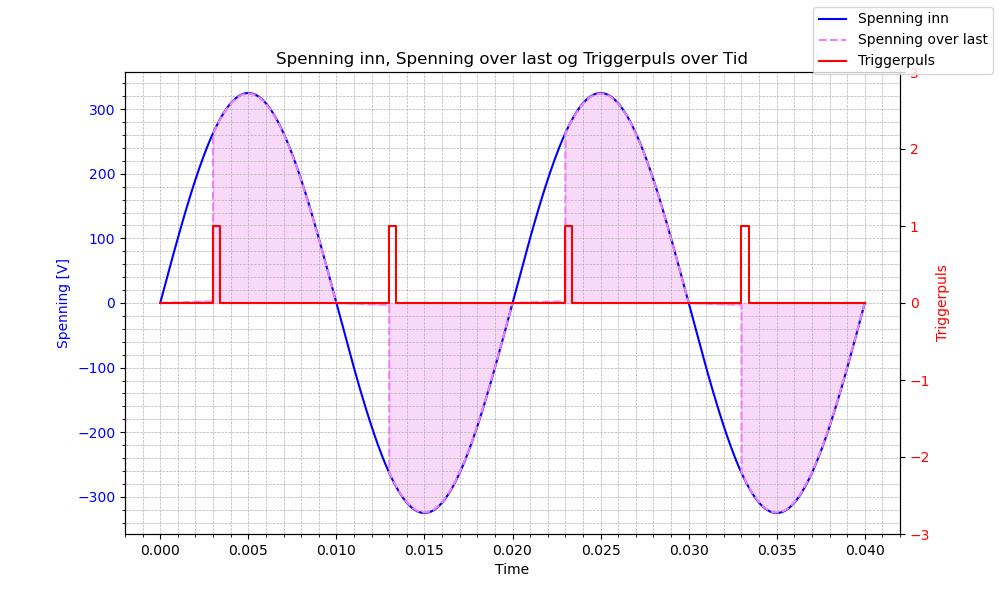
\includegraphics[width=0.9\textwidth]{tyristor/plot/triacSOL.png}
		\caption{TRIAC med trigger-signal og spenning over last}
		\label{fig:triacTriggplotSOL}
	\end{figure}

\end{solution}

% ------------------- DIAC -------------------


\begin{question}[name=Spørsmål, topic=tyristor]
	\begin{enumerate}[label=\roman*)]
	\item Hva står DIAC for?
	\item Hva er en DIAC?
	\item Hva er den typiske terskelspenningen for når en DIAC starter å lede?
	\item Hvor benytter man oftest DIACer?
	\item Hva er forskjellen mellom DIAC og TRIAC
	\end{enumerate}

\end{question}

\vspace{0.5cm} % Add space after the solution

\begin{solution}[name=Løsningsforslag]
	\begin{enumerate}[label=\roman*)]
	\item Diode for Alternating Current
	\item DIAC er en halvlederkomponent som kan lede strøm i begge retninger når spenningen over den overstiger en viss terskelverdi
	\item 30-40 [V]
	\item I sammenheng med TRIAC-er koblet på gate terminalen for å kompensere for TRIAC-ens naturlige ulikhet når det kommer til å trigge symmetrisk for både positiv og negativ halvperiode. DIAC-en vil holde igjen trigger-signalet til det er på et nivå som fører til at begge delene av TRAIC-en vil starte å lede tilnærmet momentant.
\end{enumerate}
\end{solution}

